\documentclass[tikz,border=5mm]{standalone}
\definecolor{columbiablue}{rgb}{0.61, 0.87, 1.0}
\definecolor{cyan(process)}{rgb}{0.0, 0.72, 0.92}
\usetikzlibrary{shadings}
\begin{document}
	
	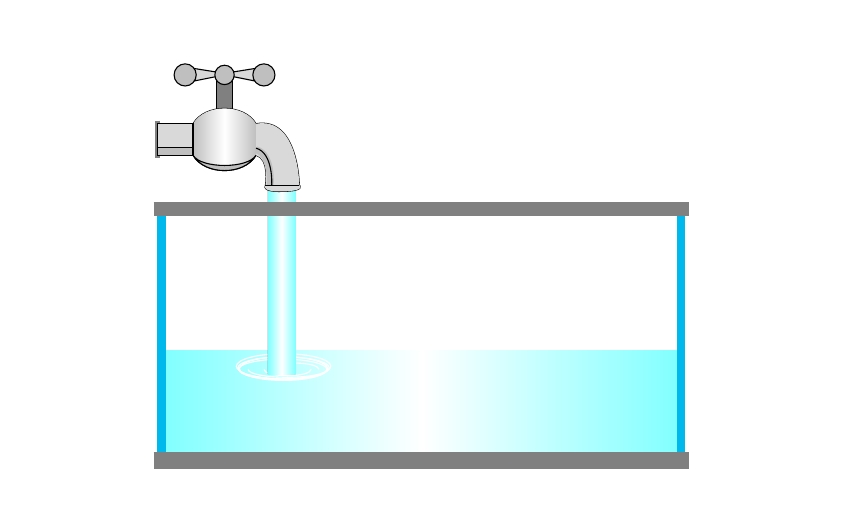
\begin{tikzpicture}
		\clip (-5,-3) rectangle (5,3);
		\begin{pgfinterruptboundingbox}
			
			\tikzset{ho_nuoc/.pic={
					%----------------------------
					
					%\fill[color=columbiablue]
					\fill[left color=cyan!50,right color=cyan!50, middle color=white](-3.3,-2.5)--(3.3,-2.5)--(3.3,-1.1)--(-3.3,-1.1);
					
					\draw[color=cyan(process),line width=3](-3.3,-2.5)--(-3.3,.7) (3.3,-2.5)--(3.3,.7);
					\draw[color=white] (-1.15,-1.3) arc (0:360:.6 cm and .16cm)--cycle;
					\draw[color=white] (-1.17,-1.32) arc (0:360:.58 cm and .14cm)--cycle;
					\draw[color=white] (-1.19,-1.33) arc (0:360:.56 cm and .15cm)--cycle;
					\draw[color=white] (-1.2,-1.34) arc (0:360:.56 cm and .13cm)--cycle;
					\draw[color=white] (-2.2,-1.34) arc (-180:0:.5 cm and .1cm);
					\draw[color=white] (-2,-1.34) arc (-180:0:.3 cm and .08cm);
					\draw[color=white] (-1.3,-1.34) arc (0:180:.3 cm and .08cm);
					\fill[left color=cyan!50,right color=cyan!50, middle color=white]
					%\fill[color=columbiablue]
					(-1.95,1)--(-1.6,1)--(-1.6,-1.4)--(-1.95,-1.4)--(-1.95,1);%nước
					%\draw[color=white] (-1.8,.5)--(-1.8,-.7) (-1.66,.1)--(-1.66,-.2) (-1.72,.3)--(-1.72,-.6) (-1.9,0)--(-1.9,-.9);
					%--------------
					\draw[color=gray,line width=5](-3.4,.7)--(3.4,.7);
					\draw[color=gray,line width=6](-3.4,-2.5)--(3.4,-2.5);
					\draw[fill=gray!30](-2.5,2.42)--(-2,2.5)--(-2,2.3)--(-2.5,2.4)--(-3,2.3)--(-3,2.5)--cycle;
					\draw[fill=gray] (-2.4,2.4)--(-2.6,2.4)--(-2.6,1.9)--(-2.4,1.9)--cycle;
					\draw[fill=gray!50] (-2.5,2.4) circle (3.5pt);
					\draw[fill=gray!50] (-2,2.4) circle (4pt);
					\draw[fill=gray!50] (-3,2.4) circle (4pt);
					%------------------------------
					\def\E{ %thân tròn vòi
						(-2.9,1.78)
						..controls +(60:.3) and +(120:0.3) ..(-2.1,1.78)--(-2.1,1.38)
						..controls +(-120:.3) and +(-60:0.3) ..(-2.9,1.38)
						;}
					\draw[color=black] \E;
					\fill[left color=gray!50,right color=gray!50, middle color=white]\E;
					\def\E{ %thân tròn vòi cong
						(-2.1,1.38)
						..controls +(-15:.18) and +(90:0) ..(-1.98,1)
						..controls +(-120:.1) and +(0:0) ..(-1.8,.92)
						..controls +(0:.35) and +(-120:0) ..(-1.55,1)
						..controls +(90:0) and +(10:.55) ..(-2.1,1.78)
						;}
					\def\F{ %đổ bóng
						(-2.1,1.38)
						..controls +(-120:.3) and +(-60:0.3) ..(-2.9,1.38)
						..controls +(-60:.2) and +(-120:0.2) ..(-2.1,1.38)
						;}
					\fill[gray!50] \F;
					\draw[color=black] \F;
					
					\draw[color=black] \E;
					\fill[gray!30] \E;
					
					\draw[color=gray!50,line width=2.5](-2.1,1.45)
					..controls +(-15:.22) and +(90:0) ..(-1.92,1);
					%\draw[color=gray,line width=1](-1.98,1)--(-1.55,1);
					\draw[color=black](-1.98,1)--(-1.55,1);
					\draw[black](-2.1,1.47)
					..controls +(-15:.23) and +(90:0) ..(-1.9,1);
					%-----------------------------------------
					\draw[color=gray,line width=1.7] (-3.35,1.82)--(-3.35,1.35);
					\draw[fill=gray!30] (-3.35,1.78)--(-2.9,1.78)--(-2.9,1.38)--(-3.35,1.38)--cycle
					;
					\draw[fill=gray!50] (-3.35,1.48)--(-2.9,1.48)--(-2.9,1.38)--(-3.35,1.38)--cycle
					;
			}}
			
			\path(0,0)pic[scale=1]{ho_nuoc};
		\end{pgfinterruptboundingbox}
	\end{tikzpicture}
	
\end{document}